%-------------------------------------------------------------------------------
% playlist
%-------------------------------------------------------------------------------
%
% \file        playlist.tex
% \library     Documents
% \author      Chris Ahlstrom
% \date        2018-09-15
% \update      2023-07-14
% \version     $Revision$
% \license     $XPC_GPL_LICENSE$
%
%     Provides a discussion of the playlist functions that Seq66 supports.
%
%-------------------------------------------------------------------------------

\section{Seq66 Play-Lists}
\label{sec:playlist}

   \textsl{Seq66} supports play-lists.
   A play-list provides a way to step through and
   play a number of MIDI files without
   having to load each one individually.
   The format of the play-list file is a variation on the 'rc' file,
   conventionally ending with the extension \texttt{.playlist}.
   It contains a number of play-lists, each described by a
   \texttt{[playlist]} section.
   Each play-list section provides
   a human-readable title which is selectable via a MIDI data number,
   or by moving to the next or previous playlist in the list using the
   \index{keys!arrow}
   \texttt{Up} and \texttt{Down} arrow keys.
   Each playlist section contains a list of MIDI files, also selectable via a
   MIDI data number, or by moving to the next or previous song in the list
   using the \texttt{Left} and \texttt{Right} arrow keys.

   Movement between the playlists and the songs is accomplished via 
   MIDI control or the arrow keys.
   Using MIDI control (\texttt{[midi-control]}, see
   \sectionref{subsec:configuration_ctrl})
   makes it possible to use the \texttt{seq66cli}
   headless version of \textsl{Seq66} in a live setting.
   See \sectionref{sec:launchpad_mini}; it describes
   programming for the \textsl{Novation LaunchPad Mini} for
   \textsl{Seq66}.
   In the normal user-interface, play-list movement
   can also be done manually via the four arrow keys on the computer
   keyboard.

   The playlist file can be specified on the command-line, in
   the 'rc' file, or be loaded
   from the \textbf{File / Open Playlist} menu or in
   the \textbf{Playlist} tab.
   The playlist setup is written to the 'rc' file; the 'rc' file
   indicates the name of of the play-list file and if it is to be used
   or not.

%  It can be removed by specifying a blank (i.e.
%  two double-quotes, "") play-list name.
%  The file extension is \texttt{.playlist}.

   The \textsl{Qt} user-interface supports editing of the play-list, using
   the \textbf{Playlist} tab.
   For version 0.99.7, this tab has been revamped.
   It was somewhat confusing to use, so the fixes make the
   process much easier.

   The user can use a text editor to edit the play-list file, if careful.
   The play-list format is defined in the following section.
   Later sections describe the user-interface.

\subsection{Seq66 Play-Lists / 'playlist' File Format}
\label{subsec:playlist_setup}

   The play-list file, by convention, has a file-name of the form
   \texttt{sample.playlist}.
   The play-list file starts with a hardwired top banner.
   It can also have an optional comments section, much
   like the 'rc' and 'usr' files.
   It is \textsl{not} overwritten when \textsl{Seq66} exits, unless it
   has been modified in the \textbf{Playlist} tab.

   \begin{verbatim}
   [comments]
   Comments added to this section are preserved....
   \end{verbatim}

   A blank line (without even a space) ends the comment section.
   Following the comments section is a \texttt{[playlist-options]} section.

   \begin{verbatim}
   [playlist-options]
   unmute-next-song = true   # the next song selection unmutes its patterns
   auto-play = true          # if true, unmute and start play automatically
   deep-verify = false       # If true, every MIDI song is opened and verified
   \end{verbatim}

   The first option allows the load of the next song to enable the patterns in
   that song (and start playing???).
   The second option causes each MIDI file to be opened to verify that it is an
   error-free play-list.  This process can be time-consuming for large
   playlists.  If set to false, \textsl{Seq66} still makes sure that
   at least each MIDI file in the play-list exists.

   Following the options section are one or more \texttt{[playlist]} sections.
   Each represents a complete play-list.
   Here is the layout of a sample playlist section.

   \begin{verbatim}
   [playlist]

   # Playlist number, arbitrary but unique. 0 to 127 recommended for MIDI control

   number = 126
   name = "Music for Serious Dogs"  # Display name of this play list
   directory = "contrib/midi/"      # Storage directory for the tunes

   # Provides the song-control number and the base file-name of each song in
   # this playlist.  The playlist directory is used, unless the
   # file-name contains a path.

   70 "allofarow.mid"
   71 "CountryStrum.midi"
   72 "contrib/wrk/longhair.wrk"
   \end{verbatim}

   \index{playlist!tag}
   A play-list file can have more than one \texttt{[playlist]} section.  This
   allows for partitioning songs into various groups that can be easily
   selected (e.g. based on the mood of the musician or the audience).

   \index{playlist!number}
   After the \texttt{[playlist]} tag comes the play-list number.
   In order to use MIDI control to select the playlist, this number
   is limited to the range 0 to 127.
   If there is more than one \texttt{[playlist]} section, they are ordered by
   this number, regardless of where they sit in the play-list file.

   \index{playlist!title}
   Next comes a human-readable name for the playlist, which is meant to be
   displayed in the user-interface.  If surrounded by quotes, the quotes are
   removed before usage.

   \index{playlist!song-storage directory}
   Next is the song-storage directory.
   This directory is the default location in which to find the songs
   in that play-list.
   It can be an absolute directory or a relative directory.
   However, be wary of using relative directories, since they depend on where
   \textsl{Seq66} is run.

   Note: If a song's file-name has its own directory component, that overrides
   the default song-storage directory.

   Lastly, there is a list of MIDI song file-names, preceded by their numbers.
   As with the playlist numbers, they are restricted to the range of 0 to
   127, for potential usage with MIDI control.
   The songs are ordered by this number,
   rather than by their position in the list.

\subsection{Seq66 Play-Lists / 'rc' File}
\label{subsec:playlist_rc_file}

   The most consistent way to specify a play-list is to add an entry like the
   following to the 'rc' file:

   \begin{verbatim}
   [playlist]
   active = true
   name = "/home/ahlstrom/.config/seq66/sample.playlist"
   base-directory = ""
   \end{verbatim}

   This setup allows a play-list file to be specified and activated.
   If the name of the play-list file does \textsl{not} contain a base-directory,
   then the play-list file is searched for in the user's \textsl{Seq66}
   configuration directory.
   If the play-list file-name is empty (i.e. set to \texttt{""}), then there is
   no play-list active.

\subsection{Seq66 Play-Lists / 'ctrl' File / [midi-control]}
\label{subsec:playlist_rc_file_midi_ctrl}

   The MIDI control stanzas for play-list and song-selection don't quite follow
   the toggle/on/off convention of the \texttt{[midi-control]} section, though
   the layout is the same:

   \begin{verbatim}
         Key   Load-by-number     Next            Previous
      24 "F2" [ 144 2 1 127 ] [ 144 4 1 127 ] [ 144 0 1 127 ] # Play List
      25 "F3" [ 144 5 1 127 ] [ 144 3 1 127 ] [ 144 1 1 127 ] # Play Song
   \end{verbatim}

   \index{arrow keys}
   \index{keys!arrow}
   Note that the key assignments are actually unused here, but the four
   arrow keys are hard-wired for use in navigating the play-lists and songs.

   Both lines specify setting the next playlist or song according to a 
   MIDI data value,
   or via "next" and "previous" controls.  The "next" and "previous" controls
   can be implemented by any MIDI event, including \textsl{Note On} or
   \textsl{Program Change}.  However, the "value" section requires a MIDI event
   that provides a \texttt{d1} (second data byte) value, such as velocity,
   because this value is
   used as the MIDI control number to select a playlist or song item.
   So, the following setting,

   \begin{verbatim}
      24 "F2" [ 0x90  2  1 127] . . .
   \end{verbatim}

   specifies that a \textsl{Note On} event with channel 0 (144 = 0x90) on note
   \#2 with a velocity between the range 1 to 127 will select a play-list.
   However, this selection will be made only if the velocity ranges from 1 to
   127, and there exists a selection with that velocity in the play-list file.
   This control requires a controller device that can be configured to provide
   the exact \textsl{Note On} event, including the exact velocity.

\subsection{Seq66 Play-Lists / Command Line Invocation}
\label{subsec:playlist_cmd_line}

   The command-line options to specify (and activate) the play-list feature
   are:

   \begin{verbatim}
      -X playlistfile
      --playlist playlistfile
   \end{verbatim}

   The play-list file is either a base-name (e.g. \texttt{sample.playlist})
   or a name that includes the full or partial path to the play-list file
   (e.g. \texttt{data/sample.playlist}).
   If no path is specified, the directory is the currently set
   \textsl{Seq66} configuration-file directory.
   For session (e.g. NSM) support, one must stick with the configuration directory;
   do not provide an explicit directory-name.

   Please note that any play-list file specified on the command line, or loaded
   in the play-list user-interface,
   will be written into the 'rc' file's \texttt{[playlist]} section when
   \textsl{Seq66} exits.

\subsection{Seq66 Play-Lists / Verification}
\label{subsec:playlist_verify}

   When \textsl{Seq66} loads a play-list file, the
   \texttt{deep-verify} option allows every
   song in the play-list file to be verified by loading it.  If any load fails,
   then the playlist will fail to load.  This check can be slow when there are
   many large MIDI files specified in the play-list file.

\subsection{Seq66 Play-Lists / User Interface}
\label{subsec:playlist_uis}

   Playlists and songs can be selected or moved-to via keystrokes or
   user-interface actions, in addition to MIDI control.

   The \texttt{Up} and \texttt{Down} arrows move forward or backward through
   the list of play-lists, and the
   The \texttt{Right} and \texttt{Left} arrows move forward or backward through
   the list of songs for the currently-selected play-list.

   The Qt 5 user-interface supports the display, selection, and editing of
   the play-lists and the song-list for each play-list.
   There are still some minor issues to work out.  If encountered, close
   \textsl{Seq66} and edit the \texttt{.playlist} file manually.
   It is self-documenting.

\begin{figure}[H]
   \centering 
%  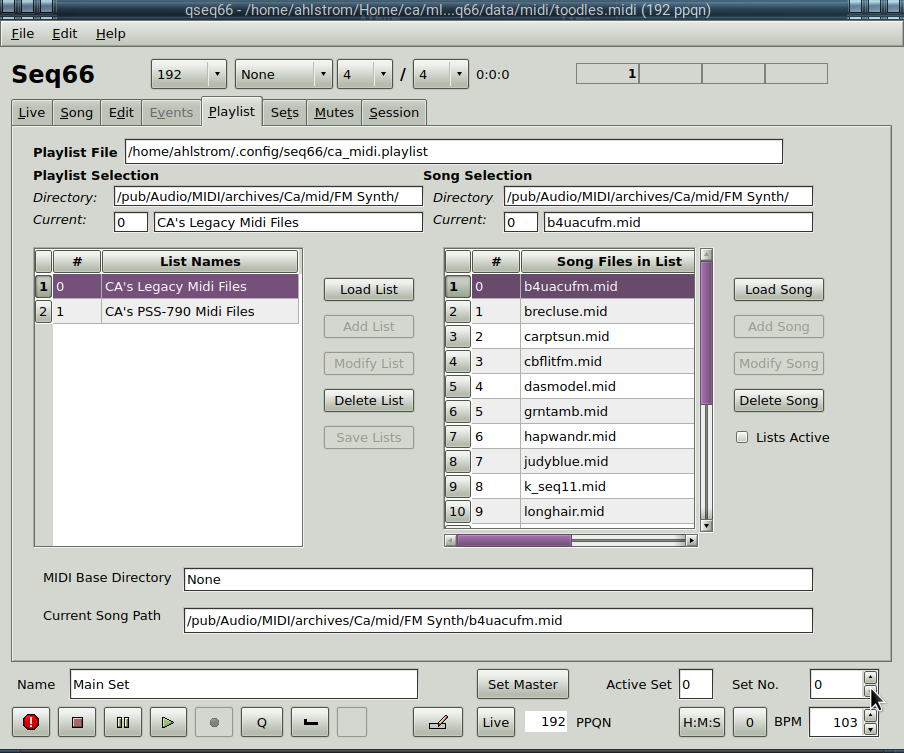
\includegraphics[scale=0.65]{tabs/playlist/personal-playlist-light.png}
   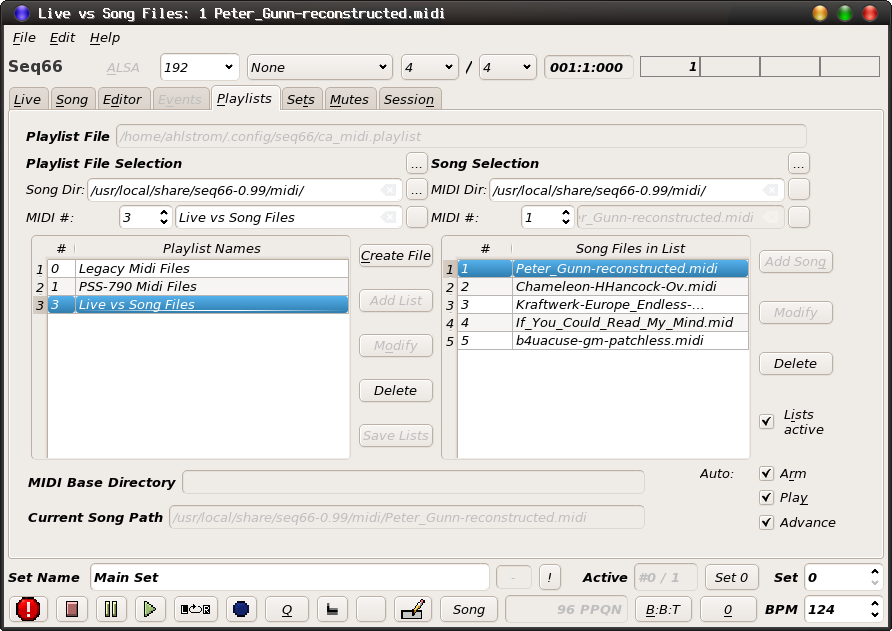
\includegraphics[scale=0.65]{tabs/playlist/personal-playlist-new.png}
   \caption*{Seq66 Playlist Tab}
\end{figure}

   There is a lot to talk about in this tab.
   It has recently been modified to some extent, so note the changes.

   Play-list specification:

   \begin{enumber}
      \item \textbf{Playlist File}.
         This field displays the path to the loaded
         play-list file.  It is not editable.  Remember that
         a play-list file can contain multiple play-lists.
      \item \textbf{Playlist File Selection}.
         These fields are editable, with the intent to use them to add a new
         play-list or modify the current one.
         \begin{enumber}
            \item \textbf{Selection}.
               This section has a button labelled \textbf{...} that
               replaces the old \textbf{Load List} button.
               It opens a file-dialog to select an existing play-list
               file, reading it in, and logging the play-list directory
               sub-play-lists into the following items.
            \item \textbf{Song Dir}.
               This field displays the main MIDI-file directory
               for the play-list currently selected in the table.
               The \textbf{Song Dir} is where the MIDI files reside by default.
            \item \textbf{MIDI \#}.
               This combo-box shows the MIDI control number for the current
               play-list, and the name of the selected play-list.
               Note that the \textbf{MIDI \#} combo-box provides values from
               0 to 127 which can be selected or edited.
               The entries are ordered by this number in the table.
               When a new play-list is specified, this number is
               set to one past the highest existing play-list number.
               It can be modified as long as it's not the same as
               another MIDI number.
            \item \textbf{Name}.
               This field shows the user's name for the selected playlist.
         \end{enumber}
%        A file-name can include a different path, however.
      \item \textbf{Playlist Names}.
         This table shows the MIDI-control number and
         the name of each play-list.
      \item \textbf{List Buttons}.
         These buttons are described below.
         See \sectionref{subsubsec:playlist_ui_playlist_buttons}.
         Please note that, in some cases, the exact functionality might
         not be perfected.
   \end{enumber}

   Song specification:

   \begin{enumber}
      \item \textbf{Song Selection}.
         These fields display the MIDI-file directory,
         the MIDI control number, and the file-name of the selected play-list.
         \begin{enumber}
            \item \textbf{Selection}.
               This section has a button labelled \textbf{...} that
               replaces the old \textbf{Load Song} button.
               It opens a file-dialog to select an existing MIDI
               file and logging the file's directory and file-name
               into the following items.
            \item \textbf{MIDI Dir}.
               This field displays the directory holding the selected
               MIDI file.
               Note that the directory is normally the play-list directory,
               but a path present in the MIDI file-name overrides that
               directory, and then an asterisk is shown to flag that status.
            \item \textbf{MIDI \#}.
               The MIDI control number field is editable,
               with the intent to use it to add a new song.
               This combo-box shows the MIDI control number for the current
               MIDI file.
               Note that the \textbf{MIDI \#} combo-box provides values from
               0 to 127 which can be selected or edited.
               The entries are ordered by this number in the table.
               When a new MIDI file is specified, this number is
               set to one past the highest existing MIDI file number.
               It can be modified as long as it's not the same as
               another MIDI number.
            \item \textbf{Name}.  
               Holds the name of the selected MIDI file.
               It is not editable because it needs to be an existing MIDI
               file.
               To assign the MIDI file a readable base name, give it a
               long file-name
               (such as \texttt{Live Play Version of Opus 11.midi}).
         \end{enumber}
      \item \textbf{Song Files in List}.
         This table shows the MIDI-control number and
         the name of each song.
      \item \textbf{Song Files in List Buttons}.
         These buttons are described below.
         See \sectionref{subsubsec:playlist_ui_song_buttons}.
         Please note that, in some cases, the exact functionality is still
         being worked out or perfected.
   \end{enumber}

\subsubsection{Seq66 Play-Lists / User Interfaces / Playlist Buttons}
\label{subsubsec:playlist_ui_playlist_buttons}

   This section briefly describes the "List" buttons to the right of the
   play-list table.

   \begin{itemize}
%     \item \textbf{Load List}.
      \item \textbf{Create File}.
      \item \textbf{Add List}.
      \item \textbf{Modify}.
      \item \textbf{Delete}.
      \item \textbf{Save Lists}.
   \end{itemize}

   \setcounter{ItemCounter}{0}      % Reset the ItemCounter for this list.

%  \itempar{Load List}{playlist editor!load list}
%  This button brings up the "Open play-list file" dialog, using the
%  \textsl{Seq66} configuration directory as the default directory.
%  It is recommended to use only this directory, especially when running in a
%  session manager. If loaded from somewhere else, save the file back to the
%  configuration directory.

   \itempar{Create File}{playlist editor!create file}
   This button brings up file dialog; one selects the desired play-list
   directory and types in the name of the new play-list file.
   The file isn't actually created until \textbf{Save Lists} button is
   clicked.

   \itempar{Add}{playlist editor!add list}
   This button is enabled with the editing of the \textbf{Playlist Selection}
   fields.  Once these three fields are correct, the new play-list can be added.
   The new play-list can then be populated with songs.

   \itempar{Modify}{playlist editor!add list}
   This button is enabled with the editing of the \textbf{Playlist Selection}
   fields.  Once these three fields are correct, the list can be modified.

   \itempar{Delete}{playlist editor!delete list}
   This button removes the currently-selected play-list from the play-list
   file.  This action doesn't take effect until the play-list file is saved or
   \textsl{Seq66} exits and does its normal saving.

   \itempar{Save Lists}{playlist editor!save lists}
   This button bring up a file dialog to save the current play-lists and songs
   into the specified play-list file.

\subsubsection{Seq66 Play-Lists / User Interfaces / Song Buttons}
\label{subsubsec:playlist_ui_song_buttons}

   This section briefly describes the "Song" buttons to the right of the
   song-list table.

   \begin{itemize}
      \item \textbf{Load Song}.
      \item \textbf{Add Song}.
      \item \textbf{Modify Song}.
      \item \textbf{Delete Song}.
      \item \textbf{Lists Active}.
   \end{itemize}

   \setcounter{ItemCounter}{0}      % Reset the ItemCounter for this list.

   \itempar{Load Song}{playlist editor!load song}
   This button bring up a dialog to open a MIDI or WRK file from
   the current song-directory or from an arbitrary directory.
   Currently, be careful with this option; adding a file from an arbitrary
   directory will generally prepend that directory to the MIDI file-name,
   making the song list difficult to read.

   \itempar{Add Song}{playlist editor!add song}
   This button is meant to add a song already loaded in the \textbf{Live} frame
   into the play-list.  Just open a new tune, test it, and then add it to the
   play list.  Note that currently one may load a new tune into the playlist
   from anywhere a song is allowed to be loaded by the session.

   \itempar{Modify Song}{playlist editor!modify song}
   This button is meant to modify song information.  However, the only item
   that can be altered is the MIDI control number.

   \itempar{Delete Song}{playlist editor!delete song}
   This button deletes the currently-selected song from the song list.

   \itempar{Lists Active}{playlist editor!lists active}
   If checked, the play-list is enabled, and the arrow keys, automation keys,
   and MIDI controls (if configured) can be used to move between play-lists and
   songs.
   Note that this check-box will not work unless there are play-lists and songs
   that exist in the tables and on the computer's file system.

\subsubsection{Seq66 Play-Lists / User Interfaces / Info Fields}
\label{subsubsec:playlist_ui_info_fields}

   The following read-only fields show some information about the file-system
   for the play-lists.

   \begin{itemize}
      \item \textbf{MIDI Base Directory}.
         Provides the top-most directory where all of the files in the
         play-list are stored.
         Currently read-only, in order not to interfere with session locations.
      \item \textbf{Current Song Path}.
         Shows the exact path the the currently-selected song.
         Currently read-only, in order not to interfere with session locations.
   \end{itemize}

   These items can be modified, however, by editing the play-list file
   directly.

   In addition, the following check-boxes set a couple of play-list features.
   
   \begin{itemize}
      \item \textbf{Lists active}.
         This items reflects the status of the play-list being active as
         configured in the 'rc' file.
         When a new play-list file is created, this item can be check-marked
         if the play-lists and their songs are basically valid.
      \item \textbf{Auto: Arm}.
         This item sets the \texttt{unmute-next-song} (unfortunate name!)
         item in the 'playlist' file.
      \item \textbf{Auto: Play}.
         This item sets the \texttt{auto-play} item in the 'playlist'
         file. If set, the the \textbf{Arm} setting is automatically set as
         well. When set, the next song starts playing as soon as it
         is loaded.
      \item \textbf{Auto: Advance}.
         This item sets the \texttt{auto-advance} item in the 'playlist'
         file. If set, the the \textbf{Play} and \textbf{Arm}
         settings are automatically set as well.
         When set, at the end of one song, the next song is automatically
         loaded and played as well.
   \end{itemize}

   There is currently no \texttt{deep-verify} check-box; edit the 'playlist'
   file directly.

\subsubsection{Seq66 Play-Lists / Creating a Playlist File}
\label{subsubsec:playlist_creating_playlist_file}

   The "programmer's method" for creating a play-list file is simply to copy
   one and carefully modify it in a nice programmer's editor.
   This section describes creating a new play-list in the \textbf{Playlist}
   tab.  We might add pictures are some point.

   Let's assume this is the first run of \textsl{Seq66}.
   The file \textsl{qseq66.rc} is not created until after the first
   run exits.
   However, the configuration directory
   \texttt{\textasciitilde/.config/seq66/} is created at startup.
   Also, the default play-list file is set as

   \texttt{\textasciitilde/.config/seq66/qseq66.playlist}.
   This file starts as a skeleton file, containing no play-lists.

   But on our first run, we want to build a play-list, "from scratch",
   using the set of sample files files installed in
   \texttt{/usr/share/seq66-0.99/midi}.
   Start \textsl{Seq66} and select the \textbf{Playlist} tab.
   Note the \textbf{Playlist File} is set to
   \texttt{\textasciitilde/.config/seq66/qseq66.playlist}, and
   there are no play-lists and songs present.
   For this mini-tutorial we \textsl{ignore}
   the \textbf{Playlist File Selection}
   button (labelled \textbf{...}).

   Click the \textbf{Create File} button.
   A file dialog comes up; it shows the default directory
   \texttt{\textasciitilde/.config/seq66/}, and the default file
   \texttt{qseq66.playlist}.
   For this tutorial, type in the file-name
   \texttt{tutorial.playlist}.
%  Obviously, we have created the directory
%  \texttt{\textasciitilde/.config/seq66/tute/} ahead of time.
%  Select the \texttt{tute} directory and change the
%  \textbf{File name} to \texttt{tute.playlist}.
   Click \textbf{Save} button.
   \textsl{Seq66} attempts to load the play-list file, but it
   does not yet exist.
   \texttt{\textasciitilde/.config/seq66/tutorial.playlist} is
   shown in the \textbf{Playlist File} field.

   Now click the \textbf{Song Dir} button,
   and navigate to the
   \texttt{/usr/share/seq66-0.99/} directory and select the
   \texttt{midi} directory.
   Just select this directory, do not descend into it.
   Click \textbf{OK} or \textbf{Choose}.
   Change the play-list \textbf{Name} from
   "midi MIDI Files" to "Installed MIDI Files".
   The \textbf{Add List} button becomes enabled; click it.
   
   Click on the \textbf{Song Selection} button.
   Navigate to where the desired play-list MIDI files are stored
   (the previously selected \texttt{midi} directory).
   Select the first desired MIDI file and click \textbf{OK} or
   \textbf{Open}.
   If it's the desired directory and file,
   then click the \textbf{Add Song} button.
   If the MIDI file's directory is \textsl{not} the same as the play-list's
   \textbf{Song Dir},
   the song's \textbf{MIDI Dir} field holds the MIDI file's
   path, and there is an asterisk to indicate it's a
   MIDI-file-specific directory.

   Add more songs and play-lists as desired.
   Note that the \textbf{MIDI \#} number self-increments, but
   these can later be modified.
   Next, click
   \textbf{Lists active} to enable the new lists.
   Click \textbf{Auto arm} if desired.
   Click \textbf{Save Lists}.
   If desired, open the new play-list file in a text editor
   and see what it looks like.

%  Save list needs to make the playlist directory and properly write
%  the file to it. (No, we can't make a new directory here, only
%  look for it.)

\subsubsection{Seq66 Play-Lists / Playlist Sample}
\label{subsubsec:playlist_playlist_sample}

   This section describes the sample play-list that accesses the MIDI data
   files installed in
   \texttt{/usr/share/seq66-0.99/midi}.

   TODO

%-------------------------------------------------------------------------------
% vim: ts=3 sw=3 et ft=tex
%-------------------------------------------------------------------------------
